\documentclass[twocolumn]{article}
\usepackage[font=small, labelfont=bf]{caption}
\usepackage{sectsty}
\usepackage{dblfloatfix} 
\usepackage{fixltx2e}
\usepackage{graphicx}
\usepackage{color}
\usepackage[letterpaper, margin=0.75in]{geometry}
\usepackage{amsmath}
\usepackage{amsfonts}
\usepackage{tikz}
\usepackage{pgfplots}
\usepackage{parskip}
\usepackage{multicol}
\usepackage{wrapfig}
\usepackage[compact]{titlesec}
\usepackage{float}
\usepackage{pdfpages}
\usepackage{euler}

\begin{document}
\graphicspath{ {Images/} }
\sectionfont{\fontsize{11}{0}\selectfont}
\setlength{\headsep}{0pt}

\titlespacing{\section}{0pt}{*0}{*0}
\titlespacing{\subsection}{0pt}{*0}{*0}
\titlespacing{\subsubsection}{0pt}{*0}{*0}

\setlength{\parindent}{0pt}

\title{Algorithmic Biosynthesis: Staged Glycan Assembly}
\author{Anjali Jaiman and Mukund Thattai}
\maketitle

\section*{Introduction}

O-glycan synthesis is ubiquitous \cite{Apweiler1999} and well conserved \cite{Varki2009} across eukaryotes, and yet, sequencing efforts have revealed tremendous structural innovation and diversity. Eukaryotic o-glycans are composed of a small set of conserved monosaccharides and sugar linkages \cite{Adibekian2010} [Figure 1A], and mainly decorate the extracellular surface of membrane bound and secreted proteins. The enzymes catalyzing o-glycan synthesis are also mainly conserved across eukaryotes with few innovations or loses \footnote{but in multicellular organisms appear to have undergone many duplication events [\textbf{cite}]}. Thus, both the monomers and the orderings of pairs of monomers is largely conserved; o-glycan structural diversity  does not stem from diverging sets of biosynthetic reactions; instead it comes from the branched nature of glycans-- the potential structural diversity of branched molecular assemblies is orders of magnitude larger than linear molecules of a similar size. 

O-glycans also appear to take on significant and new functional roles in eukaryotes, particularly in multicellular organisms. They can serve as population \textbf{[citations]} or species markers \textbf{[citations]}, preventing cross-fertilization [\textbf{citations}] and self-targeting by the immune system [\textbf{citations}]. Glycans can also display tissue-specific glycosylation patterns \cite{Cole2012}, and to mobile cells in adults  \textbf{[cite]}. Glycans also may also indicate cell-state \textbf{[cite]} or cell-health \textbf{[cite]}. Thus glycan diversity is not only noisy expression of non-specific enzymes, but even the number of unique glycan determinants (oligosaccharide motifs that act as ligands for various glycan binding proteins). 

As information storing molecules, glycans should be synthesized in a stereotyped and reproducible manner. And indeed, in spite of glycan ubiquity and diversity, eukaryotes manage to make heterogeneous, yet stereotyped glycosylation displays which serve as cell identity and cell state markers. Misexpression of glycans are implicated in cancers \cite{Vankemmelbeke2016, Lloyd1996}, pathogenic infections [\textbf{references}] and genetic disease \cite{Freeze2011}.

However, unraveling the functional role of glycans in a cell has been hampered by a lack of understanding of how a cell manages to control the biosynthesis of these identity encoding molecules. Biological systems employ a variety of strategies to efficiently and reproducibly construct a set of molecules while minimizing incorrectly synthesized by-products. For the synthesis of linear molecules, like DNA, RNA or proteins, information about the primary sequence is directly templated in the genome. For many metabolites, structural information is encoded in the synthesis pathway, through substrate-specific enzymes or finely tuned kinetics. Glycans are synthesized through the sequential action of glycosyltransferases (GTases) in the ER and the Golgi, and like other metabolites, the products are encoded in the kinetics and topology of the biosynthetic reaction network.

The enzymes involved in o-glycan biosynthesis have a minimum substrate specificity of acceptor and donor monosaccharide types, and linkage specificity. GTases transfer a single donor monosaccharide to an available acceptor monosaccharide on the growing glycan, catalyzing a covalent bond between a particular pair of carbons on the two sugars [Figure 1B]. In addition to this minimum local specificity, a glycosyltransferase can have additional substrate specificity, inhibited and/or activated by specific glycodeterminant motifs on the growing glycan. Some GTases appear to be sensitive to the entire structure [B4GALT3] or a particular oligosaccharide motif on path from the acceptor monosaccharide to the root [B4GALNT2, GCNT4]. This kind of ``pre-node" [Fig 1C] specificity is very common in N-glycans but less so in O-glycans.  Other GTases appear to have no sensitivity to the preceeding structure, glycoslyating ``locally," where-ever there is an available carbon on the acceptor monosaccharide [A4GNT, ST3GAL2, B3GAT2, B4GALT1, ST6GAL1  \cite{Blixt2008}] or with "post-node" specificitiy, glycosylating acceptor monosaccharides that have a particular oligosaccharide motif attached to them [GCNT3,B3GALNT2,FUT4, FUT7, FUT9]. 

In available microarray analyses of GTase specificities, it appears that unlike core n-glycosylation, o-GTases recognize a host of different substrates. Much of this binding appears to be hierarchical--meaning that different substrates have different reaction rates. Although there are no comprehensive databases, it appears that many o-glycosylation and terminal glycosylation enzymes have ``post-node" and ``local" specificities [Figure 1D]. However, in spite of the growing availability of glycan microarrays that can be used to test GTase relative reaction rates and specificities, in vivo kinetics and specificities are certainly not well-measured. Thus in this work, we assumed that all enzymes-substrate interactions have identical reaction kinetics and have only local specificity (although the principles described also apply to post-node enzymes). Finally, we ignore possible heterodimer reaction units that would add an


Post-node and local enzymes have the potential to be highly promiscuous. For example, there are enzymes that glycosylate the acceptor monosaccharide at both the root and on a complex glycan structure [B4GALT1-4].  \footnote{There are other kinds of enzyme specificities that we have mostly ignored in our analysis. We have ignored enzymes that appear to be sensitive to the distance between the acceptor monosaccharide and an inhibiting or activating motif  [ST3GAL1, ST6GALNAC1, ST6GALNAC2 (?)]. We have also ignored enzymes that have selectivities dependent on complicated interactions between pre and post node sugar motifs. The first enzymatic reaction, which anchors a monomer to a serine or threonine amino acid residue on the protein, are often specific to particular peptide motifs [GALNT1-20]. GTases which extend the glycan structure can have substrate specificity that includes }








\begin{figure*}
    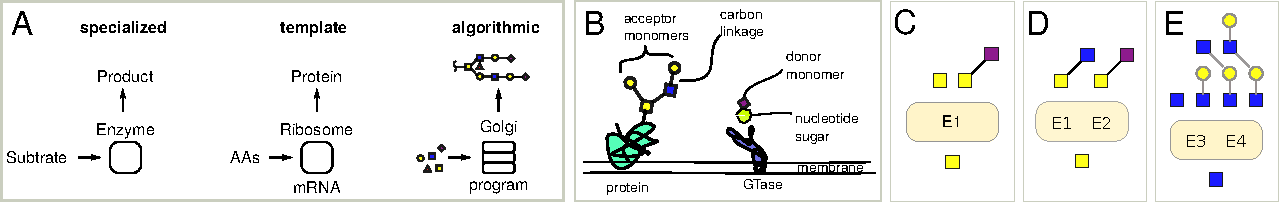
\includegraphics[width=\textwidth]{Figure_1.pdf}
	\caption{A) O-glycosylation mainly takes place in the Golgi apparatus. Proteins from the ER are shipped to the Golgi apparatus, where they are glycosylated before they are transported to the plasma membrane.  B) Locally acting enzymes. B) A glycan is an oligosaccharide. A GalNac monosaccharide is covalently attached to a serine or threonine residue on a glycoprotein. Each monosaccharide ring has multiple carbons that can bind to other monosaccharides. This allows glycans to branch. C) In the Golgi apparatus GTases transfer a single donor monosaccharide from a nucleotide sugar onto an acceptor monosaccharide on the growing glycan. Most GTases have a minimal specificity of donor, acceptor and carbon pair linkages. D) Some GTases common to mammals [see Supplemental Figure 1 for full reaction network]}
\end{figure*}

Such substrate flexibility may mean that the potential set of structures is very diverse, and gives a cell flexibility to sythesize many different kinds of glycans from the same set of enzymes and monomers. However, it is difficult to understand how a cell might control the set of final glycan products synthesized by such enzymes. For a long time cell biologists studying the Golgi have mused that the cisternae of the Golgi apparatus provides a natural staging environment to order glycosylation reactions \cite{Dunphy1985}. Although it has been difficult to find localization tags on Golgi resident proteins [cite] that would enable targeting to a particular cisternae, there is evidence that many of the enzymes required for glycosylation are targeted to a particular cisternae of the Golgi. Here we ask first, how might cells generate diversity from such limited materials. Then we ask, what is the relationship between the topology of a reaction network (i.e. the relationships between a set of coexpressed enzymes) and the observable (high abundance) diversity of products.  Finally, we ask how might compartmentalization allow a cell to construct a heterogeneous but limited set of glycans.

\section*{Sources of Diversity}
The conservation of monosaccharide types and glycosyltransferases across eukaryotes begs the question: where does glycan structural diversity come from? Some observed diversity derives from the stochastic nature of glycosylation.  Many proteins will pass through the Golgi without saturating all possible reactions, resulting in a slew of biosynthetic ``intermediates" [Figure 1B].  

\begin{figure*}
    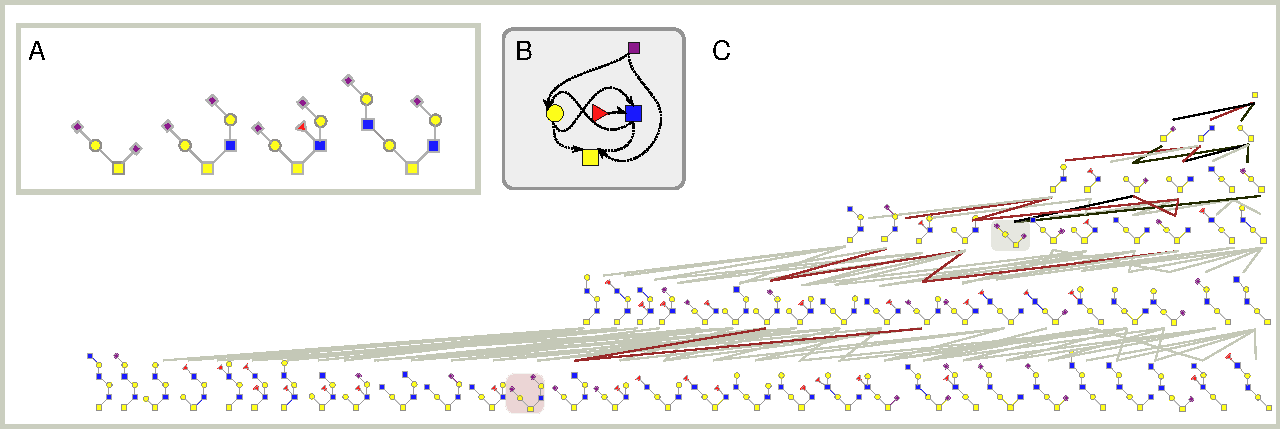
\includegraphics[width=\textwidth]{Figure_2.pdf}
	\caption{A) Sources of diversity: Incompleteness B) Sources of diversity: Competition. C) Sources of diversity: Polymerization.}
\end{figure*}

Glycan heterogeneity is also directly encoded in the topology of the reaction network. For example, the colocalization of competitive enzymes---two or more enzymes that recognize the same substrate but are mutually exclusive in their action---can contribute significantly to the richness of glycan products. For example, when two local enzymes recognize the same unglycosylated carbon on the same acceptor monosaccharide [Figure 1C],  random encounters of the substrate with either enzyme, results in a heterogeneous product set [Supplemental: Competition].

Substrate promiscuity in a reaction network also can contribute to product diversity in o-glycan biosynthesis, especially through polymerization. In Figure 1D enzyme E3 recognizes the product of enzyme E4 as its substrate, and similarly E4 glycosylates the product of E3. Cyclic motifs in a reaction network result in a vast (potentially infinite) array of glycans of different lengths and contribute significantly to the diversity of glycan product set. 

These sources of diversity are present in many reaction networks but are amplified in glycans because of branching. If the ordering of glycan branching is indiscriminate, it is represented as a partial order in the reaction network. Such substrate branching significantly increase the number of possible unsaturated intermediates over a linear structure of the same size [Supplemental: Branching]. Branching can also combinatorially increase the number of acceptor monosaccharides available to competing glycans, leading to many different chimearic structures.\\ 


\section*{Residence Times and Glycan Distributions}
The topology of the reaction network and the input substrates exactly predict glycan diversity. However, topology alone does not predict high abundance species. We calculated the closed form solutions for a family of one-parameter probability distributions to examine the relationship between reaction network topology (species diversity), species abundances and residence time. Glycan synthesis is not an equilibrium assembly problem; instead, a stable distribution of glycans is fixed by removing structures from the synthesis environment. Thus, the set of high-yield (observed glycans) will depend on the average amount of time a protein spends in the Golgi apparatus before shipment to the plasma membrane ($\tau$) [Supplemental: Reaction Network Modelling].


\begin{figure}[h]
    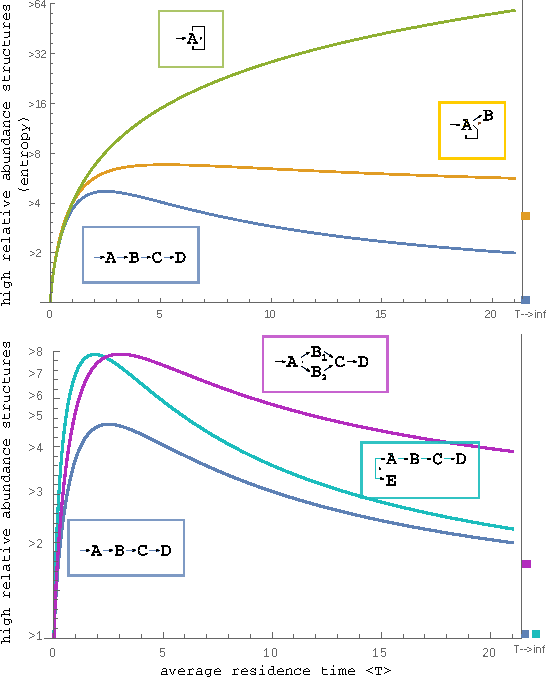
\includegraphics[width=0.485\textwidth]{Figure_3.pdf}
	\caption{A)Entropy as a function of residence time comparing a cyclic reaction network (blue), a cyclic reaction network with a competing tip (red) and a totally ordered reaction network (orange). B) Entropy as a function of average residence time comparing a totally ordered reaction network (orange), a partially ordered reaction network (light blue), and totally ordered reaction network with competition (green).}
\end{figure}

The entropy of the product distribution derived from a simple cyclic motif rises as a function of the average residence [Figure 2A, blue]. The probability distribution generated by this reaction network is exponential, and the undecorated protein is always the highest abundance product. However, as the average residence time increases, the probability distribution ``smears out" and the relative differences in abundances drop [Supplemental: Probability Distributions]. Thus, with a simple cyclic reaction motif, maintaining a very short residence time ($\tau <1 $) is the only way to limit observable heterogeneity. Even with such a generative program and a short residence time, the highest yield product will always be the undecorated form. This program cannot be tuned to maximize the yield of a chosen set of structures or to eliminate other smaller and/or larger polymeric products. 

A cyclic reaction network with a competing tip, on the other hand, will asymptotically approach a finite entropy as a function of average residence times  [Figure 2A red]. This is surprising because like the simple cyclic motif it also has an infinite number of unique potential products. However, a competing tip in this reaction network tends to act as a cap. Upon encountering a cap, a substrate becomes fixed as a terminal structure. Thus at long average residence times the distribution approaches a fixed exponential distribution without the ``smearing" described above [Supplemental: Probability Distributions]. This reaction network at long residence times, generates only a few relatively high abundance structures. However, like the simple cyclic reaction network, it is not tunable to a particular subset of structures without high yield of smaller structures and often of longer polymeric products. 

In a totally ordered reaction network, the entropy peaks and then falls again to zero at long residence times [Figure 2A orange]. If transiting proteins are exposed to the Golgi for a very short period (less than the average waiting time for a single reaction), reactions do not have sufficient time to occur, and most proteins remain undecorated [Supplemental: Abundances]. Given a long residence time ($\tau >$ L, where L is the maximum number of reactions), a majority of glycans in proceed to completion, and a single terminating structure can be observed in high abundance. Entropy peaks at intermediate residence times ($\tau\approx\frac{L}{2}$), when the expression of unsaturated structures is maximized. Thus a single terminal species can be constructed in high yield by an ordered reaction network with long residence times, on the other hand, a combination of unsaturated and terminal species can be generated at intermediate residence times. 

Competition in a totally ordered reaction network results in more unsaturated intermediates leading to a higher peak entropy [Figure 2B, green]. At long residence times, multiple species can be found as the terminal high abundance structure and so the entropy does not go to zero at long times. A reaction network with competition at long average residence times can be driven to produce a few high yield structures. At intermediate residence times, an assortment of unsaturated structures can be generated.  

Partial order, like competition also has a greater number of unsaturated intermediates than a totally ordered reaction network with the same number of reactions; thus, the maximum entropy is higher for partially ordered reaction network. Since there is only a single terminal structure, entropy approaches zero at long residence times. However, it drops off faster than a totally ordered reaction network because the multiple tips of a structure allow enzymes to parallelize their action on multiple branches. Since there are multiple attachment sites, at long residence times it is unlikely that there are asymmentric extensions, so the probability of finding these intermediates decreases.

Residence time not only works to tune the observable heterogeneity (i.e. the number of high abundance glycan structures), it also can alter the set. This effect is particularly obvious in partially ordered and competitive reaction networks, in which some predicted structural intermediates are never present in high abundances, and some are observable only at particular residence times [Supplemental:Abundances]. Even with very simple reaction network motifs with identical enzymatic rates, the set of observable structures can be significantly altered by changing the residence time.\\



\section*{Compartmentalization}
As discussed above, the diversity of a glycan product set depends on the topology of the reaction network. Therefore, we decided to examine a specific set of glycans that were likely simulatenously produced by a single biosynthetic program [Supplemental: Single Structure Simulations]. The four structures shown in Figure 3 are observed attached to a particular protein \cite{Hard1992} and are likely all simulatenously synthesized in the same Golgi apparatus in a single cell type. 

If we assume no specificity or only post-node specificity, there is a cycle in the reaction network with a competing tip [Figure 3]. Such a reaction network should have an infinite number of potential products, and at long times will have an exponential distribution of terminal fully capped structures [Figure 4A]. There is no residence time distribution that allows us to have high abundance of only these four structures. At low residence times [Figure 4A green] most proteins remain undecorated, while at longer residence times two species are completely depleted because they are not fully capped terminal structures. When the structures of interest appeared, so too did larger polymers. 

\begin{figure}[H]
    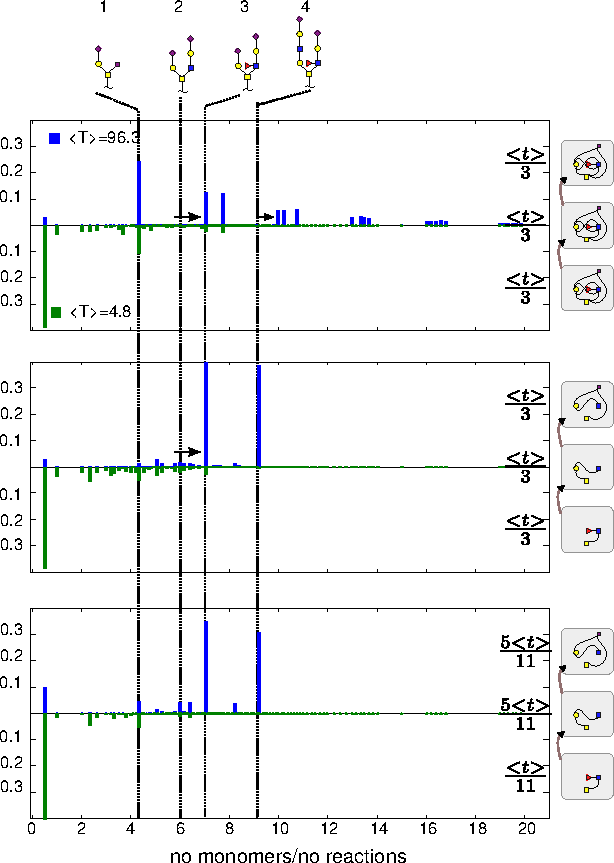
\includegraphics[width=0.5\textwidth]{Figure_4.pdf}
	\caption{A) Distribution of glycosylation products formed by putting all required locally acting enzymes in each of the three compartments. B) Distribution of glycosylation products when the required enzymes are compartmentalized according to a ``best" partition. C) Distribution of glycosylation products when the average residence times in each compartment of the ``best" partition are not taken as equal. Instead, they are taken 1:5:5. In blue, gillespe simulations were run with total average time is taken at 96.3 for each of the three programs. In mirrored plot (green), the three simulations were run with total average time at 4.8.D) Compares the KL divergences of the three programs above as the distance between a uniform distribution of the four structures and the program distribution as a function of average residence time.}
\end{figure}

In order to prevent long polymers from forming, we partitioned the reaction network into three ordered compartments [Supplemental: Compartmental Model]. We imagined that in the first compartment a set of rooted ``cores" are produced, which then act as the substrates for the reactions contained in the second compartment. The products of the second compartment then acted as the substrates of the third compartment, and the products emerging from the third compartment totaled the diversity of the program. We chose partitions that managed to produce the four observed structures, but minimized the number of additional glycans. Figure 3B shows one of the ``best" three compartmental organization, which produces 45 additional chimeras and unsaturated structures. 

Each compartment now has a subroutine that executes an acyclic reaction network. The first and second compartments are totally ordered reaction networks, while the third compartment is a partially ordered reaction network. Although there is competition in the initial reaction network, in each of these subgraphs, there are no competitive enzymes. This compartmental program prevents the formation of long polymers by partitioning the cyclic motif, and also introduces some asymmetric branch extensions by forcing further ordering on a set of partially ordered reactions.  

When we simulate the probability distribution of this partitioned program at different total residence times, at short average residence times, the there were almost no terminal species because many of the reactions in the first and second compartments do not saturate [Figure 4B green], and so the reactions in the third compartment had very low yield of reactable input substrates. At long residence times, structures 1 and 2 were complete depleted [Figure 4B, blue]. This is because at longer residence times, the products coming out of each compartment are the terminal products of that ordered or partially ordered reaction network; each subroutine operates in the long-time, low-entropy regime. However, to construct structures 1 and 2 with this partitioned reaction network, export from the first compartment must occur in the peak entropy regime, with unsaturated intermediates in high abundances, so that they can enter the second and third compartments as substrates. 

The solution to boost the yield of all structures simulatenously, requires the first compartment to operate in a high entropy regime, producing high yields of unsaturated intermediates, while the second and third compartment should operate in a long time limit with all reactions terminating. An arbitrary tuning of the first compartment to the second and the third can produce a high yield of all four structures, along with two additional chimeric structures [Figure 4c green]. This Fast-Slow-Slow assembly scheme results in a probabilty distribution that is closest to a uniform distribution on the set of observed structures [Figure 4D].

When we compare the entropy as a function of the residence time of the three different compartmental schemes, we can see the entropy will saturate at long average residence times, unlike a freely polymerizing reaction network without tips (green curve). However, when we compare a Fast-Slow-Slow tuning of the best three compartmental organization to a system in each the export from each compartment is the same, we can see that they cross. When each assembly stage allows equal residence time, as the total residence grows, the probably of an unsaturated structure exiting a particular compartment goes to zero, and the entropy drops. However, if you allow some compartments to allow unsaturated structures to exit by keeping the residence time low, you can maintain particular kinds of diversity in your distribution. \\


Different cell-types and organisms look profoundly different. Figure 4A shows a set of o-glycans found on equine chorionic gonadotropin. They contain a subset of the linkages found in human CG and the smallest structure is found on both cancerous and non-cancerous hCG. It is clear that equine CG has a polymerizing motif that extends right-side (carbon 6) chain asymmetrically. The polymerization suggests that there is colocalization of a Gal-transferase and a GlcNacTransferase. The asymmetry hints that there is compartmentalization that the left side was completed first and then right side polymerization was allowed or the right side was extended first and then the right side core 1 gal was added. 

Figure 4B-D show three different cancerous cell-types with different glycan expression profiles on the same recombinant MUC-1 protein. When comparing the highest yield structure of . 


\begin{figure*}[t]
    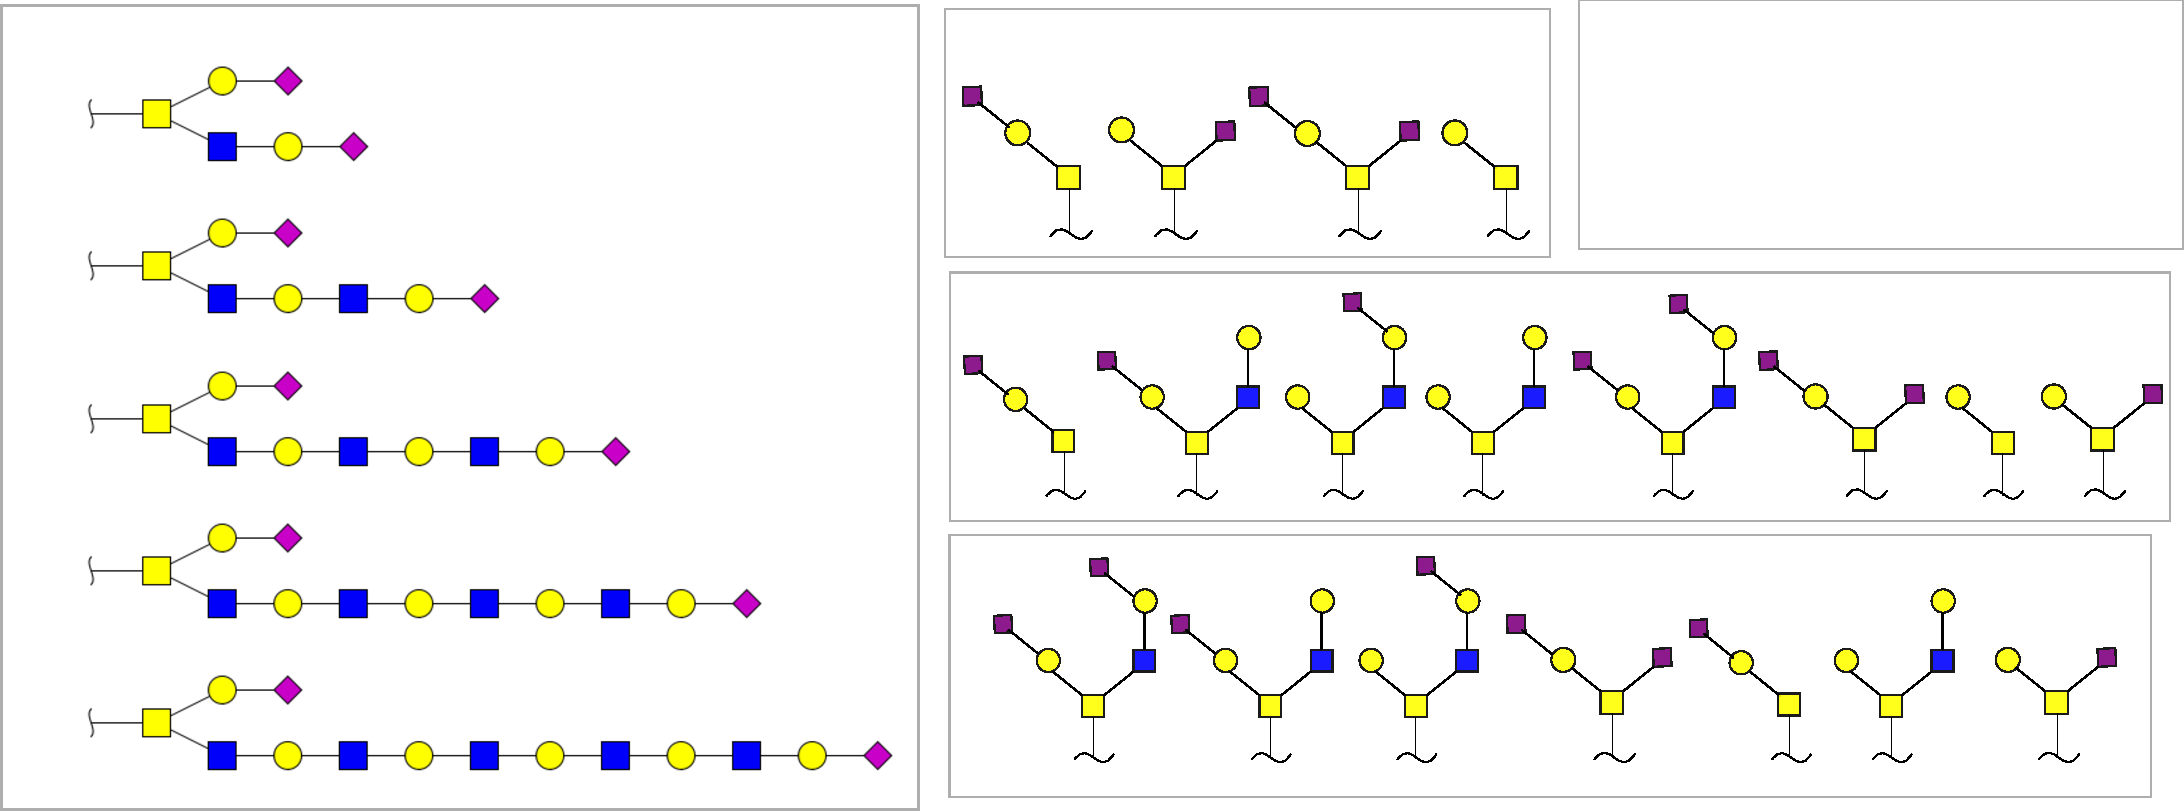
\includegraphics[width=\textwidth]{Figure_6.pdf}
	\caption{A) O-glycans found on equine chorionic gonadotropin \cite{Hokke1994}. O-glycans found on a recombinant MUC1 expressed in B) T47D, C) MDA-MB231, D)ZR-75-1 human breast adenocarcinoma cell lines \cite{Muller2002}. All structure sets contain one or more of the glycan structures found in hCG o-glycan set described above and contain a subset of the linkages found. They are ordered left to right (or top to bottom) in terms of greatest to lowest yields. Trace amounts of other species reported by \cite{Muller2002} were not included.}
\end{figure*}


\section*{Discussion}
Assembly is often framed by Winfree and others as a design problem--i.e. designing a minimial set of self-assembling building blocks \cite{Rothemund2000}, preventing kinetic trapping \cite{Fujibayashi2009, Winfree2004} and other off-target structures and developing algorithms to minimize assembly time. Our approach does not pretend to understand how the cell attempts to simulatenously optimize efficiency in time, in program size, minimize work required and minimize ``errors" in assembling the ``correct" set of structures. Instead, we consider a set of structures that likely have been assembled together in the same Golgi apparatus and we ask for stagings that can simulatenously boost the yield of that set, and minimze the yield of other structures.\textbf{Why am I actually comparing this work with other work from self-assembly literature...its actually not a contrast, we are also interested in design.} 

In general, we find that simple models of ordered reaction network partitions, with a single tunable parameter--the outshipping rate--for each compartment can help us to explain some observed glycosylation patterns [Supplemental: Additional Examples]. This is an appealing model because it does not rely on arbitrarily complex enzyme specificities, nor does it require complex tunings of different enzymatic rates to explain such rugged distributions of glycans. This model can be used to construct single structures [Supplemental: Additional Examples], as a staged assembly problem, but it can also be used to understand how heterogeneity is encoded but also controlled by an assembly program built from simple enzymes. 

This model is also appealing because of the simplicity of altering observable glycan distributions. In a single programmed partitioning, increasing or decrease the total reaction time by six fold can produce an observable different in the program output [Supplemental: KL Divergences]. Thus if the flux through the Golgi simply increases or reaction rates are decreased, the output distribution of products may change significantly.  Different proteins produced in a single cell appear to have differential rates of transport through the Golgi to the plasma membrane [\textbf{Jitu claims...find papers]}, and this could lead to heterogeneous glycosylation patterns on different proteins. Many cancerous cell types have truncated glycosylation patterns \cite{Lloyd1996}. Most research attempts to trace these altered glycan displays to abberently regulated or expressed glycosyltransferases \cite{Kannagi2009}. However, an additional possibility is that truncated glycans are partly due to increased protein flux through the Golgi or altered glycosylation rates in the Golgi \cite{Kellokumpu2002,Brockhausen2006}.

There are many human inherited diseases that cause abberent glycosylation patterns, such as cystic fibrosis, Charcot-Marie-Tooth disease, Fabry's disease and many others. These diseases do not directly mutate enzymes responsible for glycosylation. Instead they cause seemingly unrelated enzymes to be misfolded and retained in the ER. The glycosylation errors found in such diseases may instead be due to altered organization, shipping, receiving or environment in Golgi cisternae \cite{Freeze2011}. Xiang et al find that when cisternae are collapsed, the transport rate of proteins through the Golgi accelerates. Thus also results in many truncated glycoforms, although the glycosyltransferases are likely still targeted correctly to the Golgi \cite{Xiang2012}. It is possible that the abberent and excessive polymerization in cystic fibrosis and some other mucosal diseases is caused by a colocalization of a pair of polymerizing enzymes. 

Compartmental organization of enzyme serves to partition and further order a partially ordered assembly network. Alone, compartmentalization can interrupt polymerizing reaction cycles and can encode certain assymmetric branchings. This results in dramatically different probability distributions on the set of output structures depending on the specifics of compartmentalization. However, the effects of compartmentalization to encode dramatically different structure sets becomes further accentuated when kinetics are added, even in a simplistic setting in which the enzymatic rates within a compartment are tuned only to the rate of export for the compartment [Supplemental: KL Divergences]. \textbf{Stuff on pH dependent enzymatic rates?}

The notion of multifarious assembly mixtures--assemblies which can store and retrieve multiple structures built from overlapping sets of components--has been proposed by Murugan et al \cite{Brenner2015}. However, their system assumes a large number of components, and (somewhat) sparse interaction matrices. They suggest that you can retrieve a single structure from a system by tuning the chemical potentials a few interactions to generate a single nucleation seed with high probability, this then retrieves one of the many stored structures. In this problem, on the other hand, the number of components is very small, and cycles are quite likely. Indeed cycles in the reaction network are probably even required, since in certain cell-types polymers are required. Our question then becomes, how to use the small number of components to store many different structures, different subsets of which can be easily retrieved. One way to alter the program is to alter the resident times of each compartment, which generate different subsets of "seed" substrates for the subsequent compartment. 

A second mechanism to alter the set and the distribution of glycan products is to alter the compartmental partition of enzymes. A cell may want to design an algorithm for biosynthesis that maximizes the distance between two probability distributions while minimizing the number of changes in the program used to produce the probability two probability distributions. This kind of easy reprogrammability useful for a multicellular organism that needs to distinguish its different cell-types from eachCold Spring Harbor Persepctives in Biologyother, maximizing component reuse. Different cell-types can localize their glycosylaltransferases differently, and get significantly different glycosylation displays. 

What happens if the enzymes are have greater specificity than accounted for in our models? If a cyclic motif appears in a structurally derived reaction network, even if the enzymes are assumed to be post-node specific, a cycle will still appear in the reaction network, and compartmentalization (albeit a slightly different partition) can eliminate larger polymeric structures as proposed above. However, if there are indeed a significant number of pre-node or off-node specific enzymes in o-glycosylation, compartmentalization may not be required to explain observed cellular glycan displays. The problem with structurally specific enzymes--as n-glycosylation requires--is that they are not particularly flexible. The same core N-glycan appears across different cell types and indeed across many different organisms. To explain the distinct o-glycosylation patterns in different cell-types, many different highly specific GTases would have to be invoked for each glycosylation program. 

Additional points?
branching is unusual: mutual information between two branches, lower entropy, same number of reactions, parallelization. 

contrast with equilibrium calculations

deal with golgi maturation model
\bibliographystyle{plain}
\bibliography{Glycan_Paper} 

\end{document}


Measuring GTase kinetics and specificities in vivo is a challenge, making it  difficult to reconstruct network topologies or accurately predict of the observable glycan display from a cell's GTase expression profile. But biologists have taken many guesses at how a cell achieves O-glycan reproducibility. Some have argued for a strict ordering of glycan action through highly specific GTases, like those involved in N-glycan synthesis \textbf{[citations]}. Others have argued that complex hierarchieral enzyme specificites and relative kinetics can account for observed glycan data. Still others have argued that for molecular machines, in which heterdimers or larger GTase complexes can strictly order the enzymes leading to greater control over the final glycan set.  \footnote{but this doesnt really make sense to prevent wrongly ordered structures, it only speeds up the kinetics of a series reactions, you still cannot localize certain enzymes together ex. copolymerizing enzymes)} There was also the historical idea that enzyme compartmentalization in the Golgi was a plausible mechanism for ordering the structures, which has been for the most part discarded as cell biologists have come to favor the Golgi maturation model. With the exception of the compartmental ordering model, these explanations for glycan reproducibility,  heterogeneity of cell-type specific and disease glycan phenotypes are accounted for by altered GTase kinetics/specificities through genetic and epigenetic changes.


Conversely, it has been difficult to gain insights into glycan biosynthesis from glycan sequence data. Although sequencing techniques and data have been improving, mass spectrometry---the high throughput method---relies on assumptions about monosaccharide types and linkages in order to reconstruct glycan structures, and without enzyme digestion, it is difficult to assign exact branch locations to different mass fragments. Furthermore, accurate quantitative read-outs of glycan species are not easy to get and so there are potentially numerous low-abundance---and therefore unobserved---glycan structures, which makes it difficult to make any predictions about the order or the relative rates of different reactions involved in o-glycan biosynthesis. \textbf{[Make paragraph longer, with one-sentence explanation of mass spec for self-assembly crowd]}

Here, we do not argue against any of the common hypotheses about glycan biosyntheses; many of these mechanisms are probably simulatenously at play. Instead, we try to confront a simple unexplained element of glycomics hype: 
What is it about observed cellular glycan displays that is surprising? 